\newpage

 
\section{FUTURE DEVELOPMENT}

A solid and growing community is paramount to the BlockLicense success. Like any other innovation, a certain time will be needed before it penetrates the market.  The adoption period, for new technologies, looks like an ‘S’ curve \cite{pierre}, as shown in Figure \ref{fig:scurve}, where customer segmentation is spread among five main categories: innovators, early adopters, early majority, late majority and laggards.

It is expected that during the period between the pre-launch and post-launch, BlockLicense will gain market momentum, forming a noteworthy community of innovators and early adopters that will later expand to include early and late majority members. 

With an aim of achieving a 3\% of market share by the sixth year of  BlockLicense's operation, it is fundamental that  continuous marketing activities take place that focus on bringing additional value to the Blocklicense community. Activities may include incentives for both creators and buyers to use the ecosystem such as, \textit{bonus schemes} and \textit{ambassador programs} to name a few. Yet alone, marketing activities and incentives are not capable of growing or even maintaining the community. BlockLicense aims to constantly improve and expand the ecosystem by looking at community needs.

\begin{figure}[!htbp]
\centering
\begin{minipage}{1\textwidth}
  \centering
  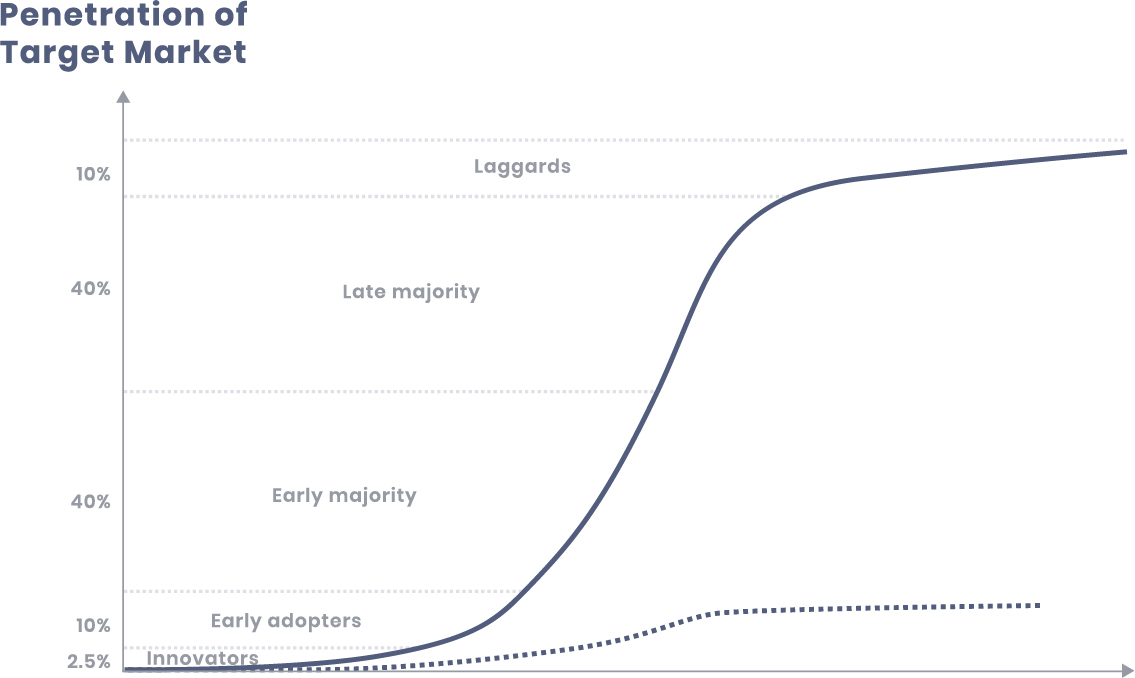
\includegraphics[width=.8\linewidth]{./figures/fig11.jpg}
  \captionof{figure}{Market Penetration.}
  \label{fig:scurve}
\end{minipage}
\end{figure}